\setauthor{Florian Beckerle}

% To Do
% Allgemeinerer Start           |
% Quellen nach jedem Absatz     |
% Rechtschreibung :(            |
%

Heutzutage kommen sich die virtuelle und die physische Realität immer näher.
Angefangen von Virtual Reality, wo sich der Benutzer mithilfe einer VR-Brille in eine fiktive Welt begeben kann,
bis hin zu Augmented Reality, in welcher virtuelle Gegenstände und Strukturen in der physischen Welt angezeigt werden können.
Es gibt neben BeamVR auch noch viele andere M\"oglichkeiten, um diese Konzepte umzusetzen zu können.
\cite{Jabil_FutureOfARVR_2021}

%Das Konzept der Synchronisation von einem Gegenstand über den zwei besprochenen Realitäten ist nicht neu.
%Einer der bekanntesten Implementierungen des Konzepts ist Richie's Plank Experience.

\section{Richie's Plank Experience}
\label{sec:richiesplankexperience}
Ein Projekt, welches zu einem Teil das gleiche Thema wie BeamVR behandelt, heißt Richie's Plank Experience, welches von TOAST VR PTY. LTD. entwickelt wurde.
Es handelt sich um ein Virtual Reality Spiel, das auf der PlayStation 4, Oculus Quest und f\"ur Microsoft Windows verf\"ugbar ist.
Bei der Playstation wird auf das Sony exclusive PlayStation VR zur\"uckgegriffen, während auf Windows entweder eine HTC Vive VR Brille oder die Valve Index verwendet werden kann.
~\cite{ToastGames_2021}

\subsection{Spielmodi}
\label{sec:richiesplankexperience_modes}
Richie's Plank Experience bietet dabei mehrere verschiedene Features in Form von Spielmodi an.
Diese Modi werden dem SpielerInnen (\"ahnlich wie bei einer Stockwerkauswahl) in einem Aufzug dargestellt.
Wenn der/die SpielerIn einen Modus ausgewählt hat, fährt der Aufzug auf das Hochhausdach.
Dort befindet sich dann der entsprechende Aufbau für den Modus.
Zur Verfügung stehen hierbei die Modi Plank, Sky Brush, Ground, Hero Academy und der Easter Egg Modus Nightmare.
~\cite{ToastGames_2021_Steam}

Im ersten Modus, welcher Plank genannt wird, befindet sich der Spieler weit oben auf einem Hochhaus.
Nach der Auswahl wird angeboten, dass sich am Ende des Balkens eine Belohnung befindet.
Man kann zwischen einem leeren Balken, Kuchen, Donuts und Kuchen mit darin versteckten Spinnen auswählen.
Nun befindet sich vor dem Aufzug nur mehr der Balken mit der vorher getroffenen Belohnung und rundherum der Abgrund.
Die Donuts und die beiden Kuchen können entweder gegessen oder heruntergeworfen werden.
~\cite{ToastGames_2021_Steam}

In Sky Brush kann der/die SpielerIn, mithilfe eines kleinen Jetpacks, frei durch die Stadt fliegen.
Dabei wird eine Rauch-Spur hinterlassen, welche, wie der Name des Modus schon andeutet, wie ein Pinsel in den Himmel malt.
Nun kann der Spieler, nach eigenem Belieben verschiedene Kunstwerke erschaffen und betrachten.
~\cite{ToastGames_2021_Steam}

Bei Hero Academy kann der Spieler wieder zwischen mehreren Optionen auswählen.
Bei Fire Deck spielt man einen Superhelden, welcher durch die Stadt fliegt und Feuer auf Häusern löschen muss.
Bei Air-Race fliegt man mit den Jetpacks durch Ringe, welche als Checkpoints für ein Rennen dienen.
Wurden alle Ringe in richtiger Reihenfolge durchflogen, hat man das Rennen geschafft.
~\cite{ToastGames_2021_Steam}

Im geheimen Modus Nightmare, welcher mithilfe des Codes 666 erreicht werden kann, erlebt der/die SpielerIn eine kleine Abfolge von gruseligen Ereignissen.
~\cite{ToastGames_2021_VivePort}

\subsection{Setup}
\label{sec:richiesplankexperience_setup}

Damit man diese Modi, vor allem den Plank Modus, mit einem realen Balken spielen kann, muss mithilfe des Setups der Balken kalibriert werden.
Hierfür wird der Balken etwa in der Mitte der VR-Spielfläche platziert.
Nun sollten beide VR-Controller auf jeweils einem Ende des Balkens platziert werden, wie in Abb. \ref{fig:beam_length_measurement} dargestellt.

\begin {figure}
    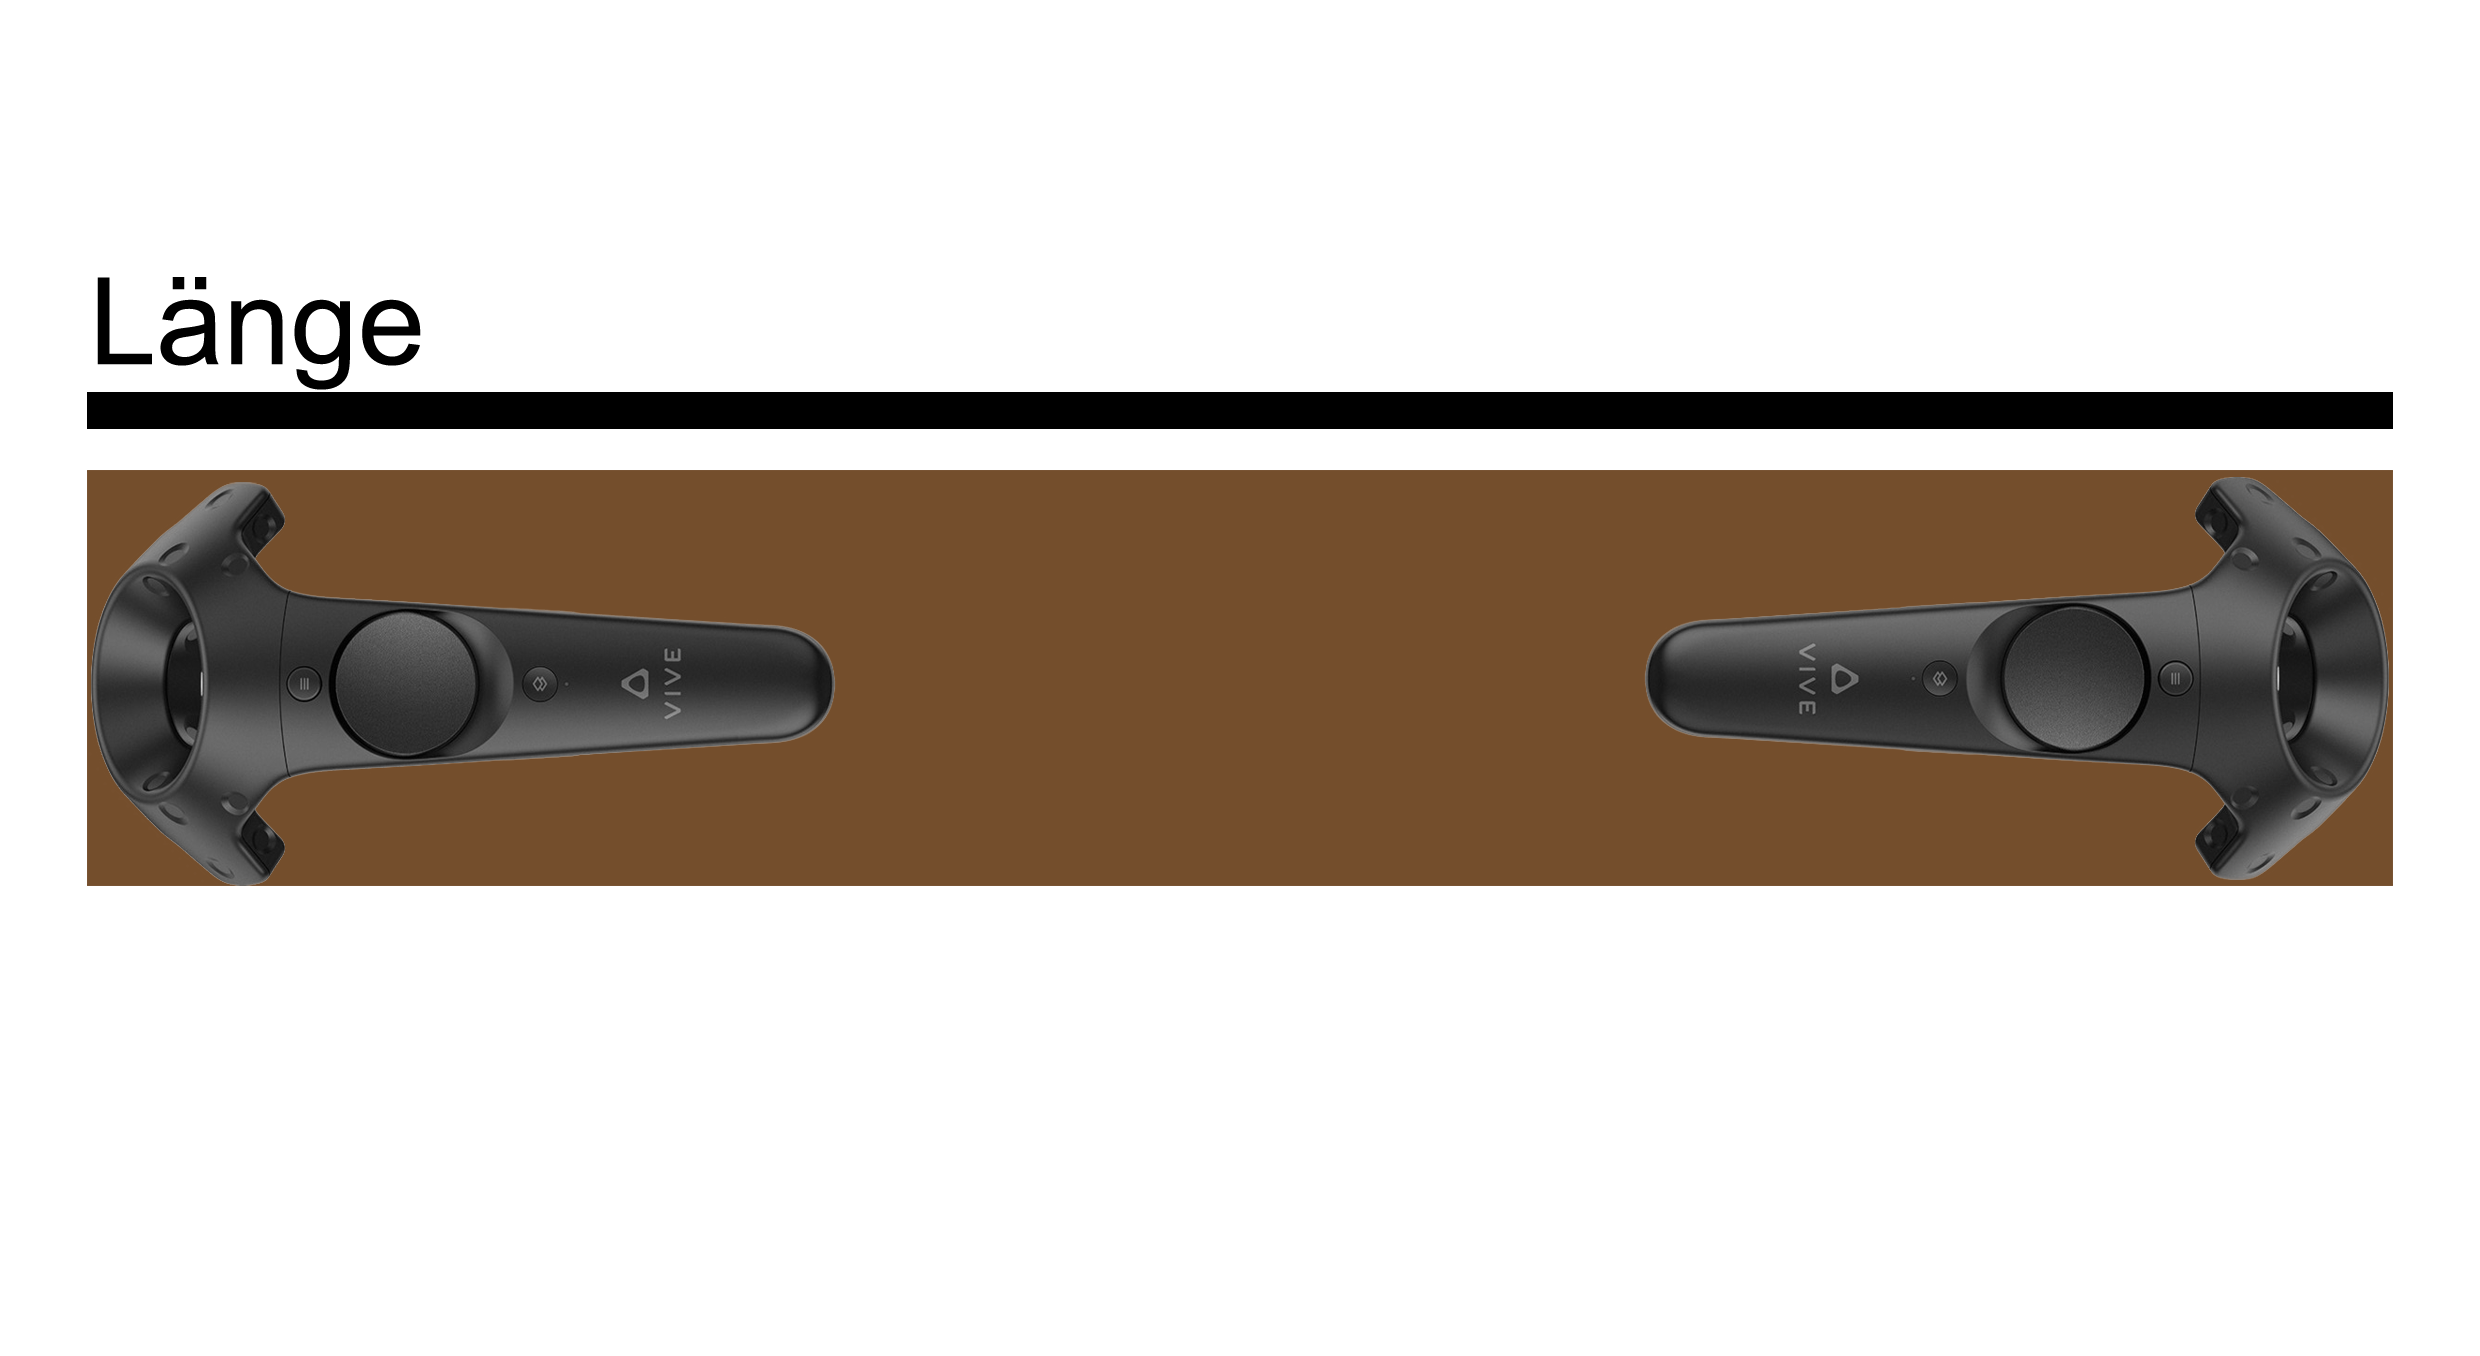
\includegraphics[scale=0.18]{pics/beam_length_measurement}
    \caption{L\"ange des Balken messen}
    \label{fig:beam_length_measurement}
\end {figure}

Dadurch weiß die Applikation wie lange der Balken ist.
Man wird aufgefordert den Trigger des Controllers zu drücken, welcher sich am Anfang des Balkens befindet, damit der Anfang und das Ende des Balkens bekannt gemacht wird.
%Grafik mit Setup Schritt 1



In Schritt zwei werden die Controller links und rechts vom Balken platziert und zeigen aufeinander.
Mit dieser Methode wird die Breite des Balkens gemessen, siehe Abb. \ref{fig:beam_width_measurement}.

\begin {figure}
    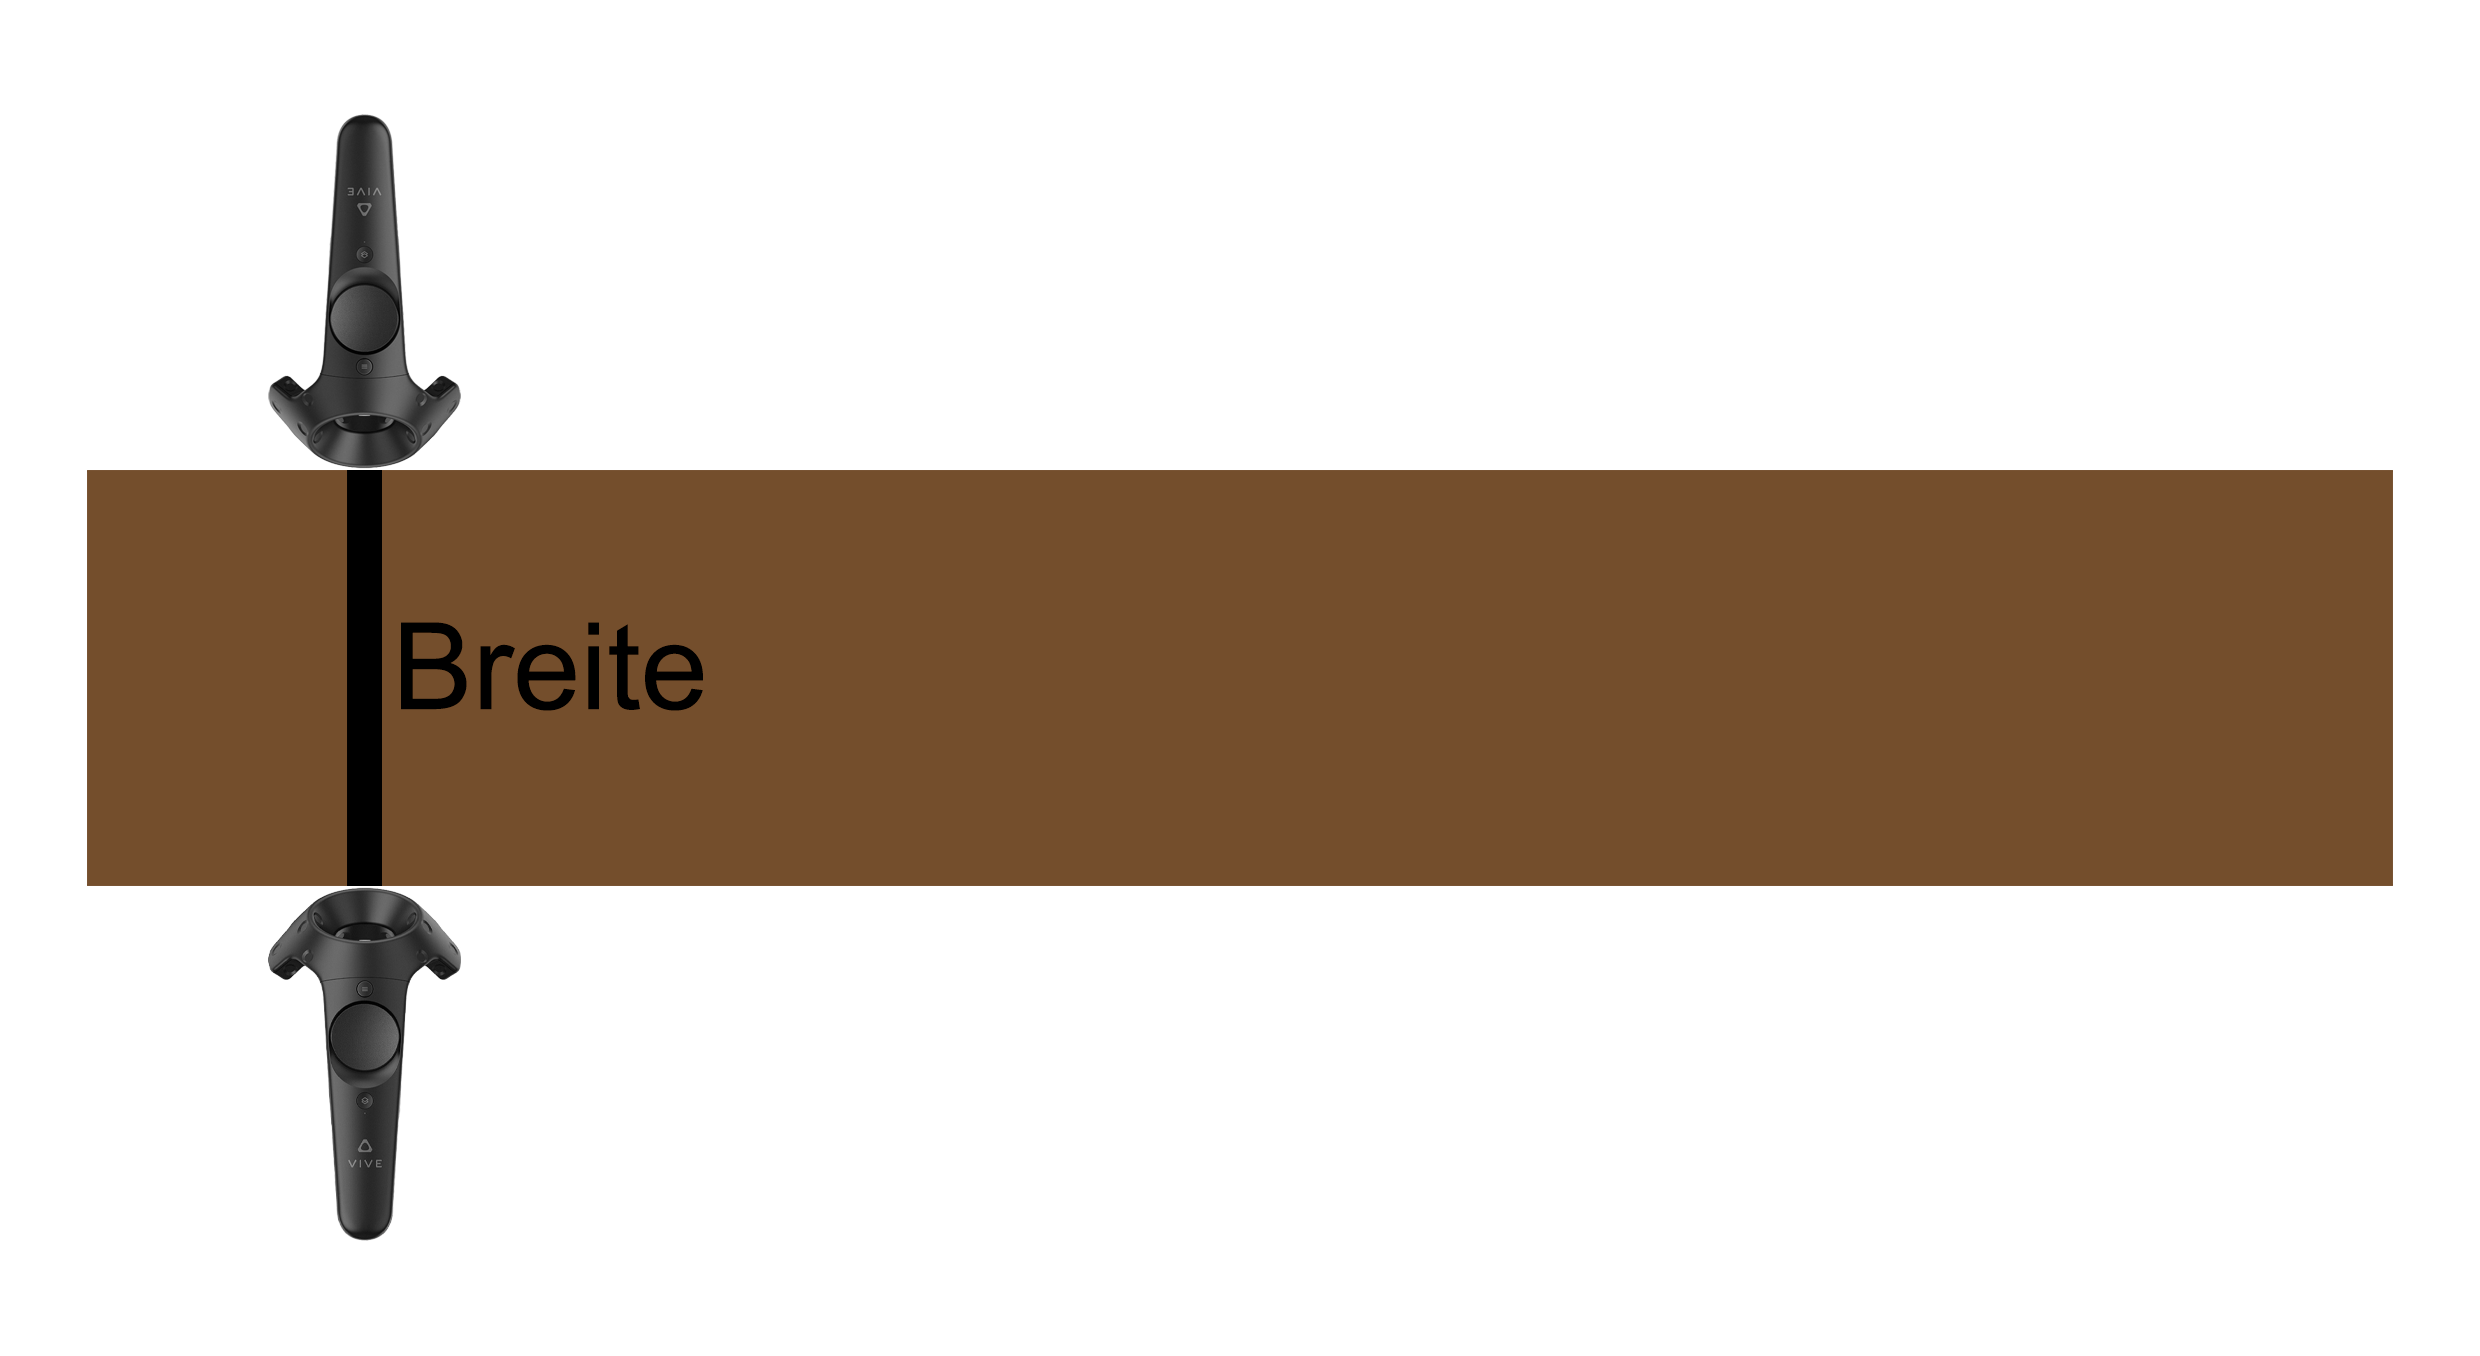
\includegraphics[scale=0.18]{pics/beam_width_measurement}
    \caption{Breite des Balken messen}
    \label{fig:beam_width_measurement}
\end {figure}


Nun ist das Setup abgeschlossen und der Balken wird richtig in der virtuellen Welt angezeigt.
~\cite{ToastGames_2021_Setup}

\subsection{Spielwelt}
\label{sec:richiesplankexperience_world}
Alle Spielmodi befinden sich in einer Stadt, welche aus einer Vielzahl an verschiedenen Gebäuden besteht.
Die Architektur ist sehr vielfältig und realistisch gehalten.
Zwischen den Bauwerken existieren Straßen, welche mit verschiedenen Pflanzen, z.B. Bäumen, geschmückt sind.
Auf Fahrbahnen befinden sich Fahrzeuge, welche mit Schritttempo durch die Stadt fahren, siehe Abb. \ref{fig:richiesplankexperience_world}.

\begin {figure}
    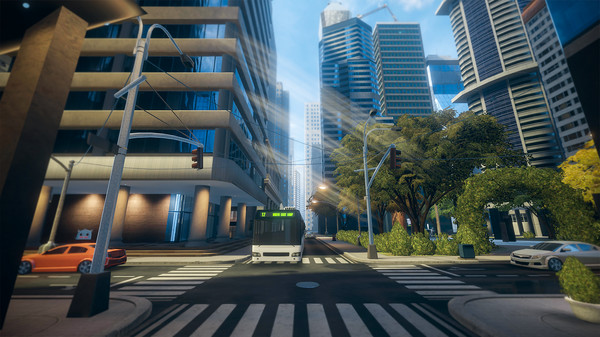
\includegraphics[scale=0.7]{pics/richiesplankexperience_world}
    \caption{Richie's Plank Experience Welt}
    \label{fig:richiesplankexperience_world}
\end {figure}


\section{VR Chat}
\label{sec:vrchat}
VR Chat befasst sich ebenfalls mit einer \"ahnlichen Thematik wie BeamVR.
In diesem Fall wird jedoch kein Balken sondern gleich wie bei BeamVR der ganze K\"orper der BenutzerInnen mit Controllern getrackt.

\subsection{Spielprinzip}
\label{sec:vrchat_principle}
Wie der Name schon sagt, handelt es sich um eine in VR ausf\"uhrbare Anwendung.
Da aber nicht jeder eine VR Brille besitzt, kann man auch eine Desktop Variante spielen, welche mit Maus und Tastatur bedient wird.
In diesem Programm geht es haupts\"achlich um die Interaktion mit unbekannten Spielern aus dem Internet,
welche ebenfalls diese Applikation verwenden.
Wer jedoch mit Freunden spielen möchte, kann das nat\"urlich auch.
Eine Vielzahl an, von SpielerInnen erstellten, Welten und Spielmodi sind bereits verfügbar und es kommen weiterhin neue dazu.
Von einer Runde Capture the flag im Weltall bis hin zu einem entspannenden Abend an einem Lagerfeuer im Wald ist alles möglich.
~\cite{VRChat_2021_Steam}

\subsection{Verwendungsm\"oglichkeiten}
\label{sec:vrchat_usecases}
Es gibt viele m\"ogliche Verwendungszwecke für eine Applikation wie VR Chat.
Die vier gr\"oßten Use-Cases dieses Programmes sind jedoch, die Option neue Freunde im Internet kennenzulernen, eigene Welten zu erschaffen,
sein digitales Aussehen selber bestimmen zu k\"onnen und Teil einer riesigen Community zu werden.
~\cite{VRChat_2021}

VR Chat ist eine soziale Plattform, auf welcher sich tausende SpielerInnen gleichzeitig befinden.
Diese interagieren in Form von Gespr\"achen oder Gesten miteinander.

Die EntwicklerInnen stellen die n\"otigen Funktionen zur Verf\"ugung, um eigene Welten zu kreieren.
Die Spieler fertigen neue Spielmodi wie z.B. Capture the flag, Lasertag, Theaterauff\"uhrungen, etc. an und errichten passende Umgebungen dazu.

Weitere Spielermodelle k\"onnen einfach mithilfe des Steam Workshops und Tools wie Ready Player Me, Tafi oder MakeAvatar, heruntergeladen und sofort im Spiel verwendet werden.
Durch dieses Feature f\"uhlt sich die Applikation sofort pers\"onlicher an, da man sich mit den Modellen besser identifizieren kann.
~\cite{VRChat_2021_AvatarCreator}

\subsection{Full Body Tracking}
\label{sec:vrchat_fullbodytracking}
BenutzerInnen, welche die n\"otigen Tracker besitzen, hierbei handelt es sich ebenso wie bei BeamVR um z.B. die Vive Tracker, können sogar seinen K\"orper und seine Beine im Spiel tracken.
Dafür sind nicht mehr als drei Schritte notwendig.


Zuerst muss man in das Men\"u des Spieles gehen und auf den Kalibrieren-Knopf dr\"ucken.

Als n\"achstes wird ein Spielermodell ausgew\"ahlt.
Dieses wird daraufhin in einer T-Pose vor dem/der SpielerIn dargestellt.
Weiters werden mithilfe von weißen Punkten die Positionen der Tracker in der Applikation angezeigt, diese sollten nun vern\"unftig platziert werden.

Zuletzt muss noch die Eingabe best\"atigt werden und das Spielermodell stellt die Bewegungen der Benutzer im Spiel dar.
~\cite{VRChat_2021_FullBodyTracking}

%\subsection{Avatar Erstellung}s
%\label{sec:vrchat_avatarcreation}
